\section{Klaus-Günther Schmidt}
\textbf{Responsibility: Android development, Bluetooth synchronization, MIDOS integration}\\
\textbf{Role: Git Master}\\

As mentioned earlier, the average palliative patient is about 70 years old. Enabling them to stay in homecare by using a mobile app with connected sensors, is a big advantage as well as a challenge.

Usually, older people are not used to interact with latest technology and due to suffering from serious diseases they often have limited mental and physical capabilities.

To deal with this problem, we decided to make the usage of our app as simple as possible. In order to support this with our implementation we focused on a simple, intuitive as well as consistent design and structure of our app.

\subsection{Prototyping with Adobe XD}
To prevent troubles when starting the actual implementation with Android Studio\footnote{https://developer.android.com/studio}, we decided to construct a mockup of our app. Therefore, I created a set of app activities, which were tested and reviewed by the other team members. This led to valuable feedback such that we were able to improve the app even before we had written a single line of code. 

We decided to create a horizontal and high fidelity prototype. The horizontal aspect means that we implement a broad overview of the app without specific, in-depth functionality. Thus, we were able to get a general overview of what the app should and might include. Furthermore, it allowed us to add or remove features with ease, not spending too much time in making things look beautiful and to ultimately identify mandatory and optional parts of our product.

A high fidelity prototype offers a realistic look and feel. This enabled us to discuss the design, layout, colors with focus on the typical capabilities and age of a palliative care patient.

To build such a mockup, we decided to use Adobe XD\footnote{https://www.adobe.com/de/products/xd.html}. It is a free-to-use tool, which has an extensive yet simple interface builder. It supports drag-and-drop to add and rearrange different shapes, text boxes, images, etc. It is possible to define common UI elements, colors as well as fonts. It even allows to model connections between the different activities so that one receives an interactive prototype.

This led to our first implementation (see Figure \ref{fig:xd}), which allowed us to continue with the planning:

 At first, we split up the app in multiple parts: Login/Registration, Homescreen, Emergency, Settings, acquiring and display of biometrical and physiometrical health information, next of kin and doctor interface. Thus, we were able to prioritize the different features. For example the acquisition and display of information as well as the emergency screen were mandatory features, while the settings and the next of kin interface were less important considering the aims of the project. Therefore, we decided to remove the doctors' interface from the Android app completely.
 
Grouping the different activities also allowed us to assign different people to the different packages so that we could implement them independently from each other.
Furthermore, we talked about the general activity design (see Chapter \ref{chap:baseactivity}) and came up with several ideas of how to keep the interface easy to understand and clean for the patients.

\begin{figure}[]
\vspace{-10pt}
    \centering
    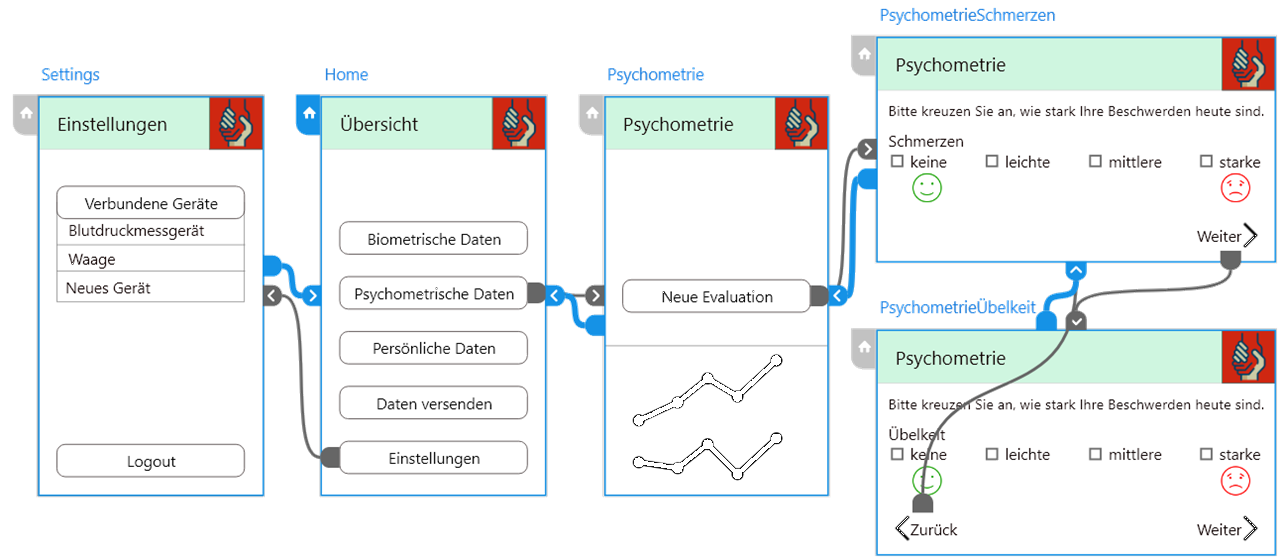
\includegraphics[width=\textwidth]{figures/KlausXD.png}
    \caption{Part of the prototype with activity connections - Screenshot AdobeXD}
    \label{fig:xd}
\end{figure}

\subsection{Defining a general app layout}
\label{chap:baseactivity}
At first, each developer started to use his own design and screen layout. By doing very similar work multiple times we were able to identify different implementation approaches for the common elements. Apart from that, we peer reviewed the different implementations. Therefore, we collected many ideas that we considered as very important.
My job was to combine all those identified aspects to be eventually able to have a common activity design as well as functionality.

Therefore, I implemented a BaseActivity class, which defines the primary visual structure of our app, featuring a help button which provides an explanation for each screen, and an emergency button to call help from any screen with only two touches.

\subsubsection{BaseActivitys}
The BaseActivity class is an abstract class which is the superclass of all of the activities for a registered user. The main purpose of the BaseActivity is to define the visual structure of these inheriting activities. This means, each activity inheriting from the BaseActivity, has the predefined main layout, but is still able to show custom text and components (see Figure \ref{fig:baseactivity}). A big advantage of this is that a future change of the common layout does not have to be done in each activity manually. Instead, it is just necessary to change the BaseActivity.

\begin{wrapfigure}{r}{0.32\textwidth}
\vspace{-10pt}
  \begin{center}
    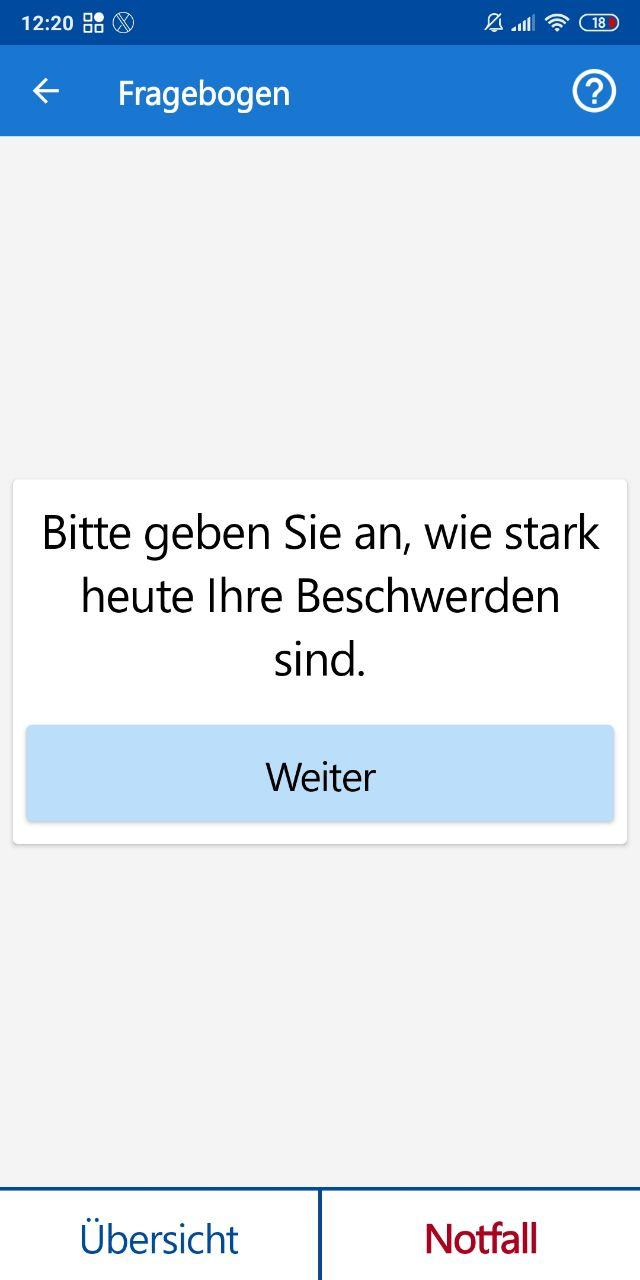
\includegraphics[width=0.30\textwidth]{figures/KlausBasicActivity.jpg}
  \end{center}
  \caption{Implementation of the BaseActivity}
  \label{fig:baseactivity}
  \vspace{-30pt}
\end{wrapfigure}
At the top of any activity, which extends the BaseActivity, is an ActionBar. The ActionBar itself is splitted into three parts: an optional back-button to access the prior activity, the title of the current activity and the help button.

For each inheriting activity it is possible to hide the back button, when it does not make sense, to change the activity title
    and to change the text which is displayed after clicking the help button.
    
At the bottom of any activity extending the BaseActivity there is a panel with two buttons: the first to return to the home screen and the second to reach the emergency activity. These buttons are very important for the patients. The home button enables them to return to the default overview screen to prevent them from being lost in the app. The emergency button enables a patient to call for help (e.g. ambulance, doctor or a next of kin) within just two clicks. 
It is possible to disable each button separately. For example in the emergency screen itself, it is not necessary to show the emergency button (see Figure \ref{fig:emergency}).

\subsubsection{Emergency Screen}
\begin{wrapfigure}{r}{0.32\textwidth}
\vspace{-30pt}
\begin{center}
    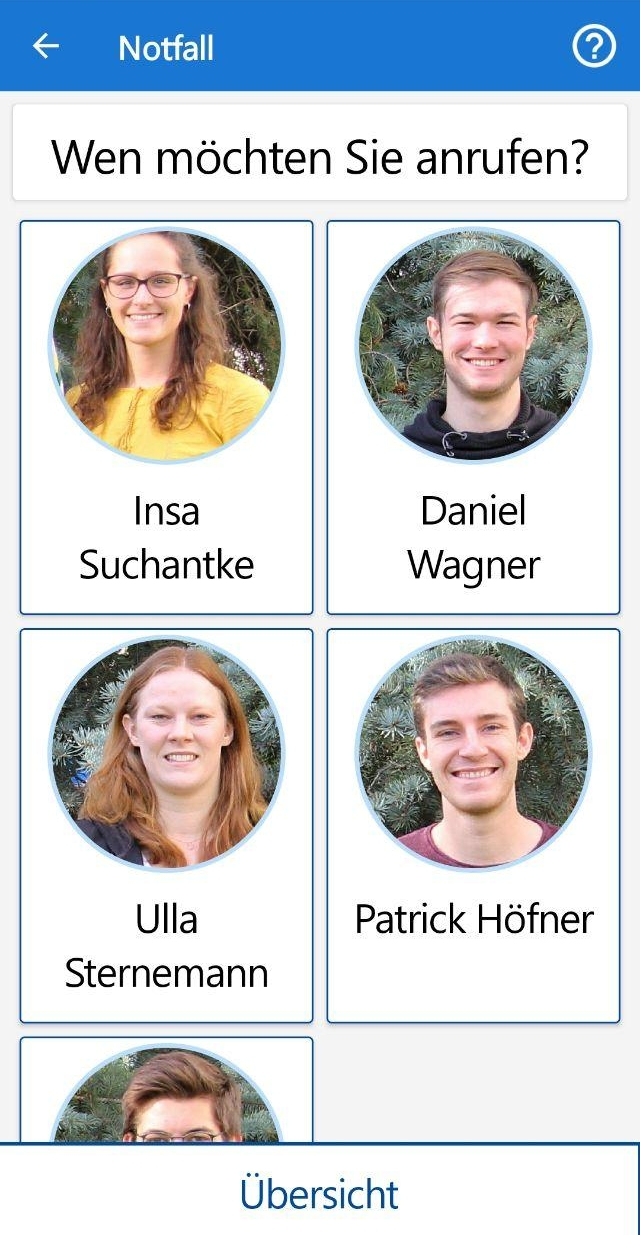
\includegraphics[width=0.30\textwidth]{figures/KlausEmergency.jpg}
  \end{center}
  \caption{Emergency Screen with Contacts}
  \label{fig:emergency}
  \vspace{-30pt}
\end{wrapfigure}
The emergency screen is a very simple to use and essential feature in our app. It enables a patient to call preassigned emergency contacts when feeling sick or suffering from exceptional pain. Each contact card consists of a (not visible) number, the name and an optional contact picture. When clicking on a contact card, the defined number is called immediately. This is realized by a simple Intent of the type ACTION\_CALL.

It was important to us that this emergency call feature is accessible in a quick way. That is why we included it in the already mentioned BaseActivity.

To be able to show the round contact images, we use the CircleImageView library\footnote{https://github.com/hdodenhof/CircleImageView} from Henning Dodenhof. It is licensed under Apache License, Version 2.0.

In the current prototype it is not possible for a patient to add custom contacts. So far only the contacts of our team are hardcoded into the app. For the following studies, the functionality will be improved to allow to add and call custom emergency contacts. Furthermore, it is planned, after clarifying the legal aspects, to include the German emergency telephone number 112 into the app as a hardcoded default "contact".

\subsubsection{Help Text}
\begin{wrapfigure}{r}{0.30\textwidth}
\vspace{-30pt}
  \begin{center}
    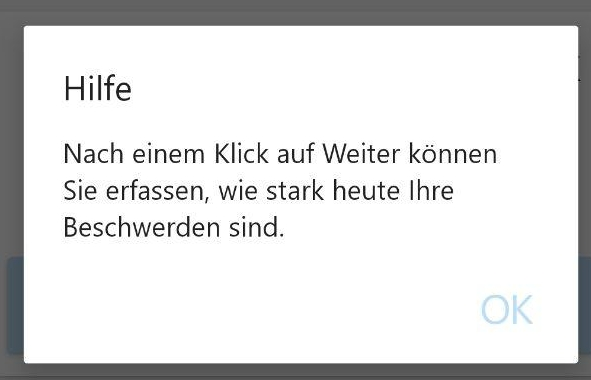
\includegraphics[width=0.30\textwidth]{figures/KlausHelpText.jpg}
  \end{center}
  \caption{Examplary help text}
  \label{fig:helptext}
  \vspace{-10pt}
\end{wrapfigure}
To provide guidance for every activity, we decided to implement the help text feature. By clicking at the questionmark button in the upper right corner (see Figure \ref{fig:baseactivity}) a new dialog is opened (see Figure \ref{fig:helptext}). The shown text can be customized per activity by overriding the abstract method getHelpText() from the BaseActivity (see Listing \ref{lst:helptext}).
 
Theoretically, there would have been an oneliner solution to set the help text by defining a string variable, which is used by the BaseActivity. However, this may result in developers forgetting to set the help text correctly. Instead, by defining the text through the implementation of the abstract method, the creator of an activity is enforced to overwrite this getHelpText() method. I have, therefore, opted for this implementation to support the developers by reminding them to set this helptext.
\begin{lstlisting}[language=Java, label={lst:helptext}, caption={Implementation of the getHelpText method in the emergency activity},captionpos=b]
    @Override
    protected int getHelpText() {
        return R.string.help_emergency;
    }
\end{lstlisting}

\subsection{MIDOS questionnaire}
The MIDOS questionnaire \cite{midos} is a brief and simple survey for the self examination of the condition of a palliative patient. It is used by several institutions, including the palliative care department of the Universitätsklinikum Erlangen. By collecting daily information of the patient, e.g. pain, nausea, anxiety or lack of appetite, it is possible to get an idea of the physical and psychological state of the patient. These aspects are very important, as palliative care deals with the "treatment of pain and other problems, physical, psychosocial and spiritual.", as defined by the World Health Organization\footnote{https://www.who.int/cancer/palliative/definition/en/}.

MIDOS consists of multiple single choice questions (up to 5 answer options) and 3 free text questions. My goal was to keep the digitized version of the questionnaire as easy and similar to filling it out with pen and paper.

The first step was to break the survey down into small parts which can be shown at the screen in a good readable font size so that the patient is not overstrained. This resulted in showing just one task at a time and a next / previous button which let the user go one step for- or backward (see Figure \ref{fig:midos1}).

\begin{wrapfigure}{r}{0.35\textwidth}
\vspace{-10pt}
  \begin{center}
  %TODO correct picture
    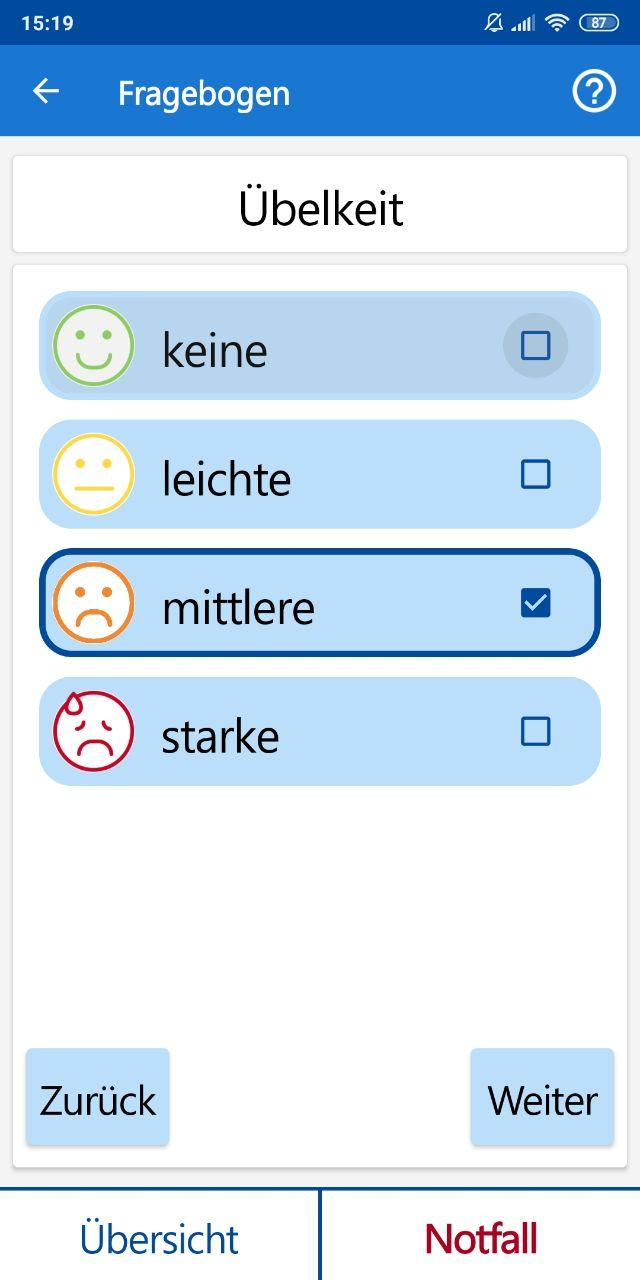
\includegraphics[width=0.28\textwidth]{figures/KlausMidos.jpg}
  \end{center}
  \caption{App version of the MIDOS survey}
  \label{fig:midos1}
  \vspace{-30pt}
\end{wrapfigure}
To achieve this, the user is guided through all questions like in a step by step tutorial. Examplary the first text is: "Bitte geben Sie an, wie stark heute Ihre Beschwerden sind." It is followed by multiple screens which look like the one in Figure \ref{fig:midos1}.
\subsection{Receiving data from a scale}
Apart from gathering psychometrical data with MIDOS, one essential functionality of our app is to acquire biometrical data of the patients through medical devices. In the first stage of our startup, we wanted to be able to demonstrate this functionality and decided to integrate a scale as proof-of-concept. One of our team members, Daniel, bought a scale from Beurer BF700\footnote{https://www.beurer.com/web/de/produkte/wellbeing/gewicht-und-diagnose/diagnosewaagen/bf-700.php} and connected to it with the help of the OpenScale project\footnote{https://github.com/oliexdev/openScale}. Since he  has taken up the task to create the webinterface, it was my job to complete the integration of the OpenScale code, and modify it to our needs. My idea was to modify the code as little as possible so 

\begin{wrapfigure}{r}{0.35\textwidth}
\vspace{-30pt}
  \begin{center}
  %TODO correct picture
    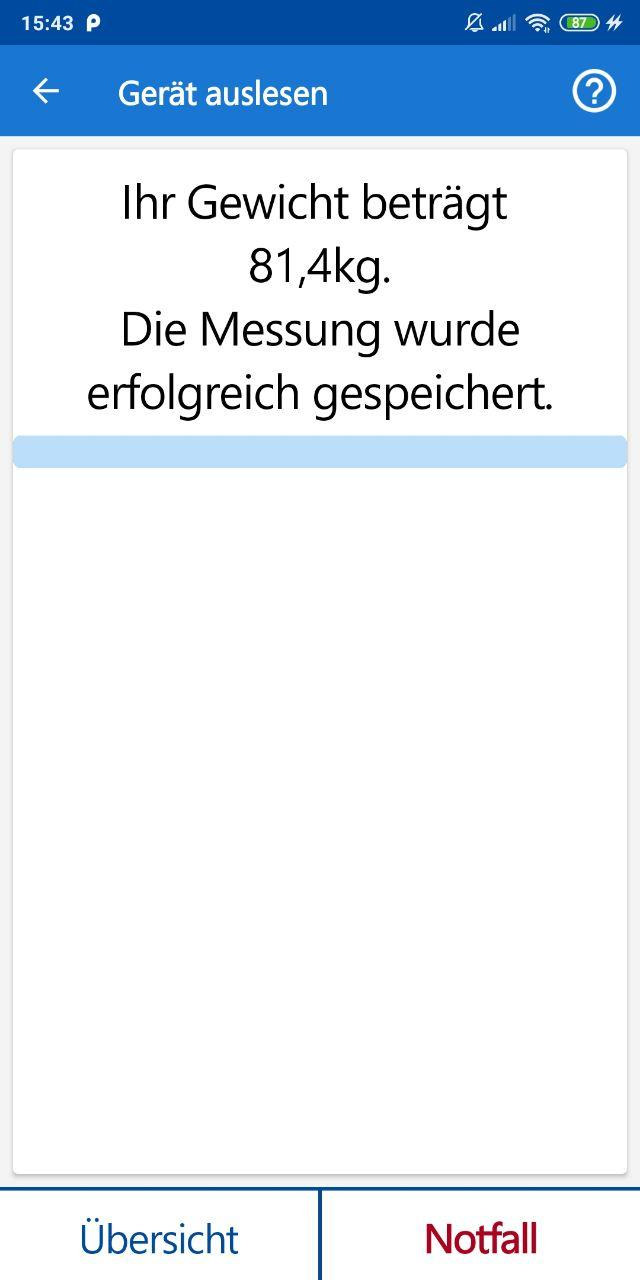
\includegraphics[width=0.28\textwidth]{figures/KlausScale.jpg}
  \end{center}
  \caption{Finished weighing}
  \label{fig:scale}
  \vspace{-10pt}
\end{wrapfigure}

that we would benefit from future updates of OpenScale without too much reworking. But yet some refactoring had to be done so that the app is reflecting the current state of the weighing process in a more adequate way. Therefore, we use a Handler as callback instance. It receives a Message object from the OpenScale classes and depending on the message state, a different action is executed. Since these messages are already sent before, during and at the end of the weighing process, we are able to lead a patient through the whole process. At first we advise the patient to switch on the scale and to step on it. After that a bar indicates the progress of the scaling and a visual, haptic (vibration) and auditive notification is raised when the weighing is done. After the process is finished, the weight is saved and displayed at the screen (see Figure \ref{fig:scale}). 